%%%
\documentclass{article}
%%%
\usepackage[x11names, rgb]{xcolor}
%%%
\usepackage{tikz}
%%%
\usetikzlibrary{decorations,arrows,shapes}
%%%
\begin{document}
%%%
% Start of code
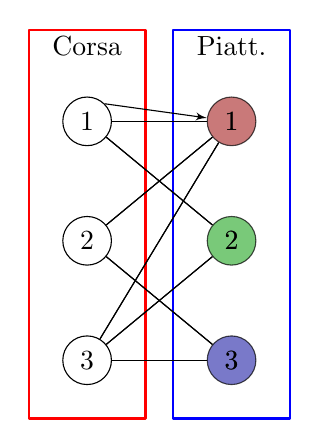
\begin{tikzpicture}[>=latex',join=bevel,scale=0.5]
%%
%%
\definecolor{c1}{rgb}{0.70,0.25,0.25}%
\definecolor{c2}{rgb}{0.25,0.70,0.25}%
\definecolor{c3}{rgb}{0.25,0.25,0.70}%
%
\begin{scope}
  \pgfsetstrokecolor{black}
  \draw[thick,red] (8bp,102bp) -- (8bp,382bp) -- (92bp,382bp) -- (92bp,102bp) -- cycle;
  \draw (50bp,370bp) node {Corsa};
\end{scope}
\begin{scope}
  \pgfsetstrokecolor{black}
  \draw[thick,blue] (112bp,102bp) -- (112bp,382bp) -- (196bp,382bp) -- (196bp,102bp) -- cycle;
  \draw (154bp,370bp) node {Piatt.};
\end{scope}
  \node (1) at (50bp,316bp) [draw,circle] {$1$};
  \node (2) at (50bp,230bp) [draw,circle] {$2$};
  \node (3) at (50bp,144bp) [draw,circle] {$3$};
  \node (4) at (154bp,316bp) [draw,circle,fill=c1,opacity=0.7] {$1$};
  \node (5) at (154bp,230bp) [draw,circle,fill=c2,opacity=0.7] {$2$};
  \node (6) at (154bp,144bp) [draw,circle,fill=c3,opacity=0.7] {$3$};

  \draw (154bp,316bp) node {$1$};
  \draw (154bp,230bp) node {$2$};
  \draw (154bp,144bp) node {$3$};

  \path[->] (1.north east) edge (4);
  \path[] (1) edge (5);
  \path[] (2) edge (4);
  \path[] (2) edge (6);
  \path[] (3) edge (4);
  \path[] (3) edge (5);
  \path[] (3) edge (6);

  \path[] (1) edge (4);
  \path[] (1) edge (5);
  \path[] (2) edge (4);
  \path[] (2) edge (6);
  \path[] (3) edge (4);
  \path[] (3) edge (5);
  \path[] (3) edge (6);

%  \draw [] (3) ..controls (92bp,265bp) and (112bp,281bp)  .. (6);
%  \draw [] (4) ..controls (95bp,144bp) and (108bp,144bp)  .. (8);
%  \draw [] (3) ..controls (95bp,230bp) and (108bp,230bp)  .. (7);
%  \draw [] (5) ..controls (92bp,93bp) and (112bp,109bp)  .. (8);
%  \draw [] (5) ..controls (82bp,86bp) and (88bp,93bp)  .. (92bp,101bp) .. controls (111bp,136bp) and (94bp,153bp)  .. (112bp,187bp) .. controls (116bp,195bp) and (122bp,202bp)  .. (7);
%  \draw [] (4) ..controls (82bp,172bp) and (88bp,179bp)  .. (92bp,187bp) .. controls (111bp,222bp) and (94bp,238bp)  .. (112bp,273bp) .. controls (116bp,280bp) and (122bp,287bp)  .. (6);
% \draw [] (1) ..controls (92bp,367bp) and (112bp,351bp)  .. (6);
%  \draw [] (2) ..controls (92bp,281bp) and (112bp,265bp)  .. (7);
%  \draw [] (0) ..controls (81bp,459bp) and (87bp,452bp)  .. (92bp,445bp) .. controls (114bp,414bp) and (131bp,375bp)  .. (6);
%  \draw [] (2) ..controls (95bp,316bp) and (108bp,316bp)  .. (6);
%
\end{tikzpicture}
% End of code

%%%
\end{document}

